% Very simple template for lab reports. Most common packages are already included.
\documentclass[a4paper, 12pt]{article}
\usepackage[utf8]{inputenc} % Change according your file encoding
\usepackage{graphicx}
%\usepackage{url}

%opening
\title{Motion Capturement Project Paper}
\author{Steven Arnow, Axel Isaksson, Markus Renström\\stevena@kth.se, axelis@kth.se, markusre@kth.se}

\date{\today{}}

\begin{document}
\pagenumbering{gobble}
\maketitle



%1. A description of the system and application you have decided to implement.  Be sure to explain why the application is useful, and how it uses sensors. Förklaras i Introduktion, Application och sensors, samma frågor som draften till proj.

%2. A complete description of the software and hardware architecture you have used to implement your project.  This description should have block diagrams of your system, hardware schematics, software flowcharts and listings, and other information about how you implemented your system and application.

%3. Data that shows how your design performs.

%4. [SHOULD BE DONE INVIDUALLY]! Conclusions about your design.  Interpret your data and describe how well the application works.  Explain performance, especially in terms of power consumption, and estimate of cost.  Critique your design.  Do you think people would buy it?  How much money might they spend to buy it?  How would you improve your design?  What would you do differently if you were to re-design it?  Be as detailed and thoughtful as you can on these points.

\section*{Introduction}
This report covers the results of a project in the course Sensor based system (II2302) at KTH during the fall of 2015\cite{kursp}. The project was to create a sensor based motion capturement system which relied on gyroscopes and accelerometers to capture and track movements of an object. The goal was to be able to record motions and capture the movements of i.e. limbs, simple objects or small animals.
%%Fyll på?

%%%%%%%%%%%%%%%%%%%%%
\subsection*{The application}
A motion capturement system \cite{wiki} can be used in many applications where real world motions and movements is studied or analysed. The most common usage for a motion capturement system is digital animation in video games and movies where characters movement is based on movements taken from a motion capturement system. The application can also be used in physics, medical implementation and sports to collect data for further analysis.

The technique behind motion capturement and recording motion have only been used for around a decade. Since the technique is rather new there's still much potential for finding new implementations in the field.
 
%%Fyll på?

    
%Applications for a motion capturement system is   we want to develop during this project is a motion capture system  that will be able to see and record movements. The idea is to develop some smaller modules which records accelerations as well as orientation and then by combining their data information about the motion can be created.

  
%%%%%%%%%%%%%%%%%%%%%
\subsection*{Sensors}
The system created in this project used mostly accelerometers and gyroscopes.  small   would most likely depend on sensors such as accelerometers and gyroscopes to capture the actual motions. The project would probably also need some sort of wireless module with radio sensors to be able to "lift out" heavier computations and avoid wires (with can prevent mobility). 

The smaller modules will therefore be connected to a larger module which will transmit the collect the data wirelessly to a computer. This will have the benefits of avoiding limitation by cables and such. 


\section*{Design}
In this part of the report all the hardware and software constructed during this project will be presented and explained. The architectures of the implementations will be shown in flow charts, block diagram, schematics to illustrate how the system is functioning.  

%%%%%%%%%%%%%%%%%%%%%
\subsection*{Block diagram}
Below is a simple block diagram presented which shows the main design of the project (see Figure ~\ref{fig:pic2}). The picture also gives a quick indication of which kinds of parts the implementation will need. The figure also shows that the hardware can be divided into three parts with different functionallity and objective.    
 
\begin{figure}[h!]
    \centering
    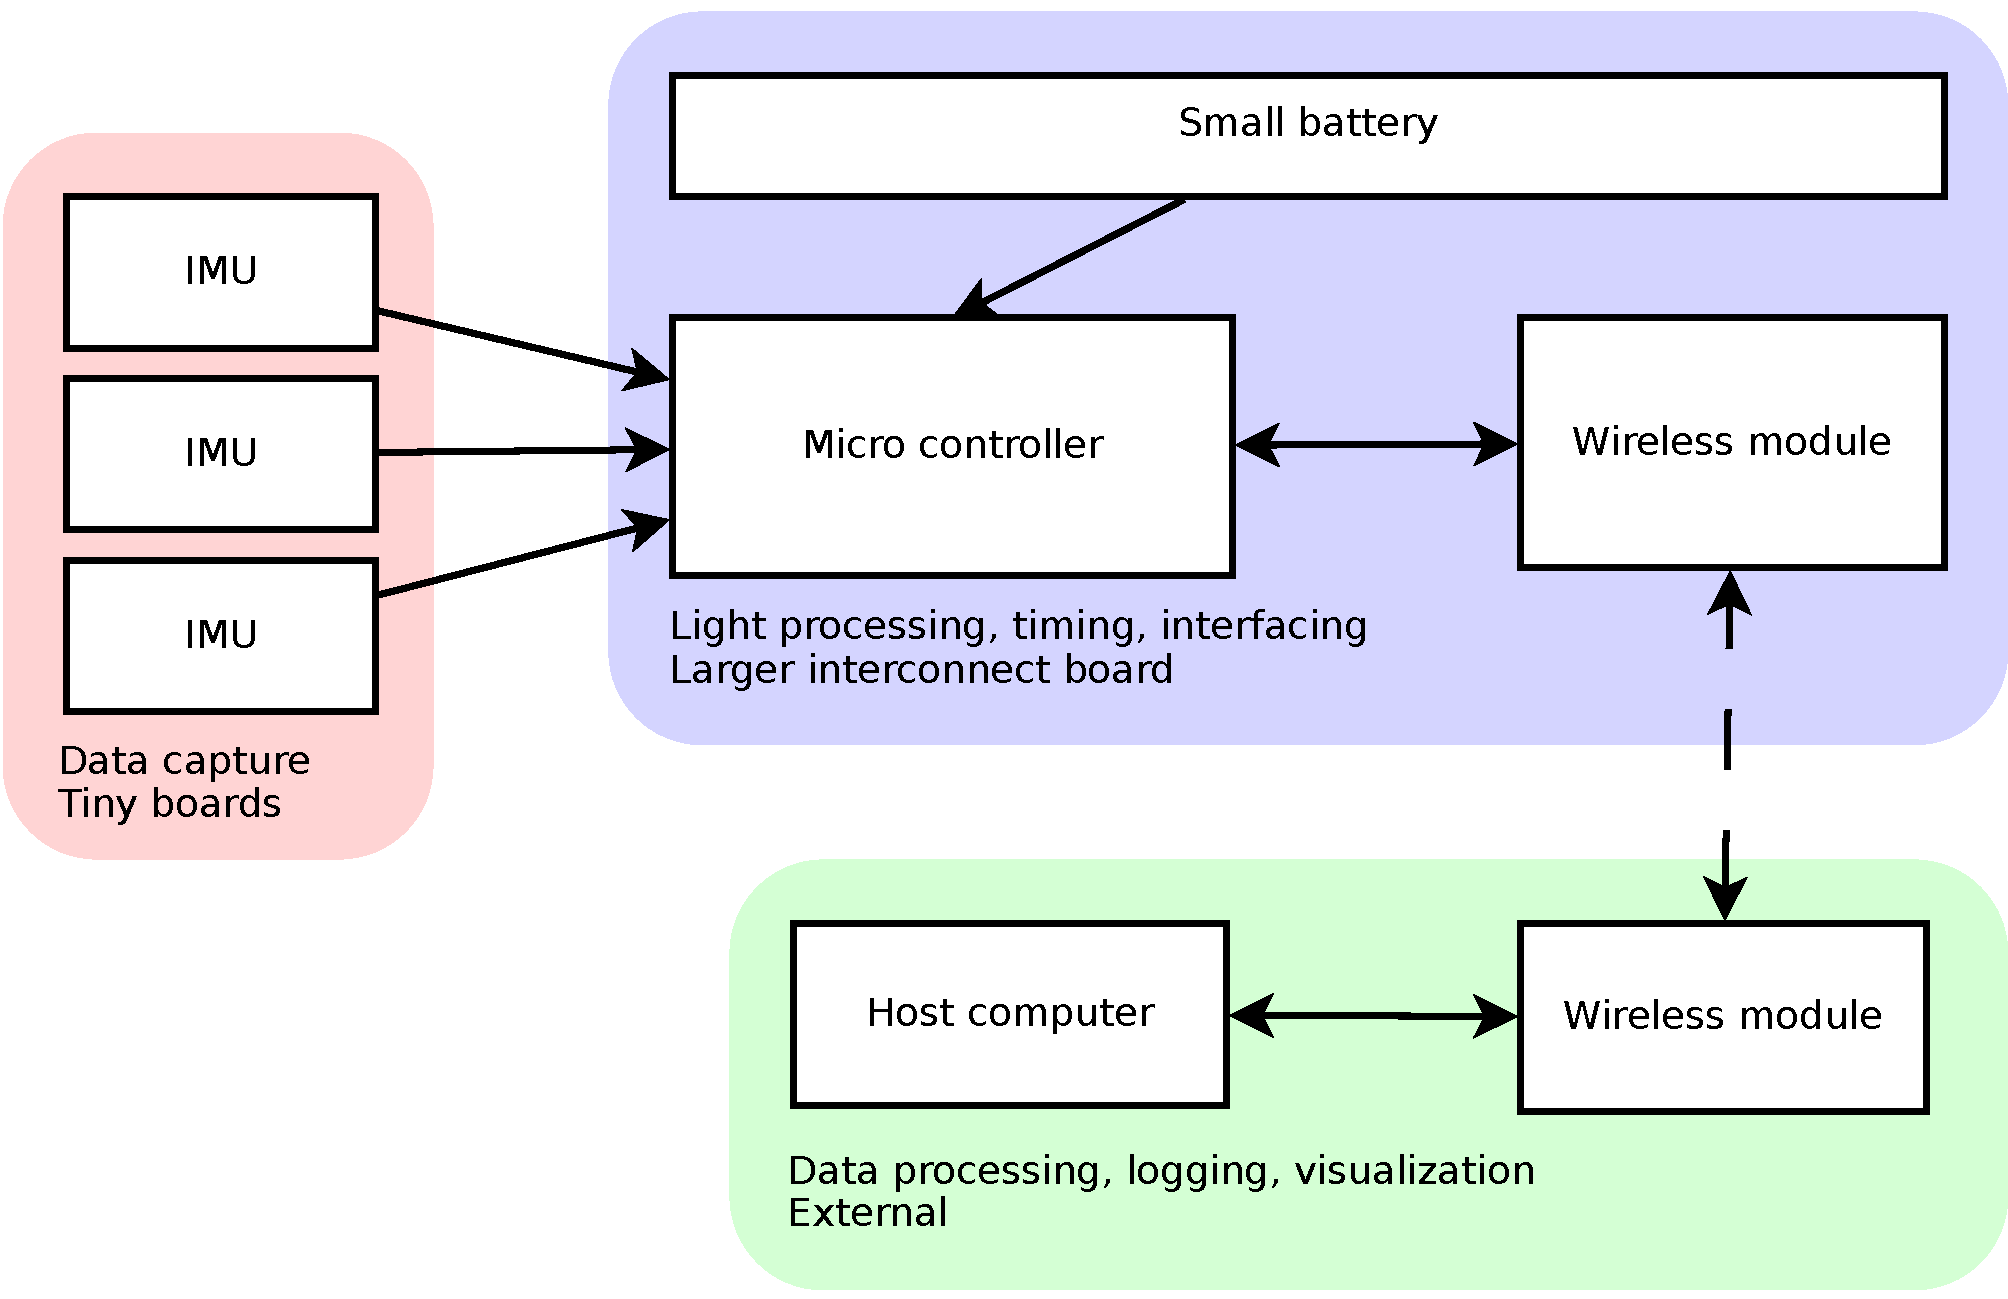
\includegraphics[scale=0.38]{block.pdf}
    \caption{A block diagram showing the most vital parts of the project, note that the different part is physically separeted.}
    \label{fig:pic2}
\end{figure}

\subsection*{Flow charts}

\begin{figure}[H]
    \centering
    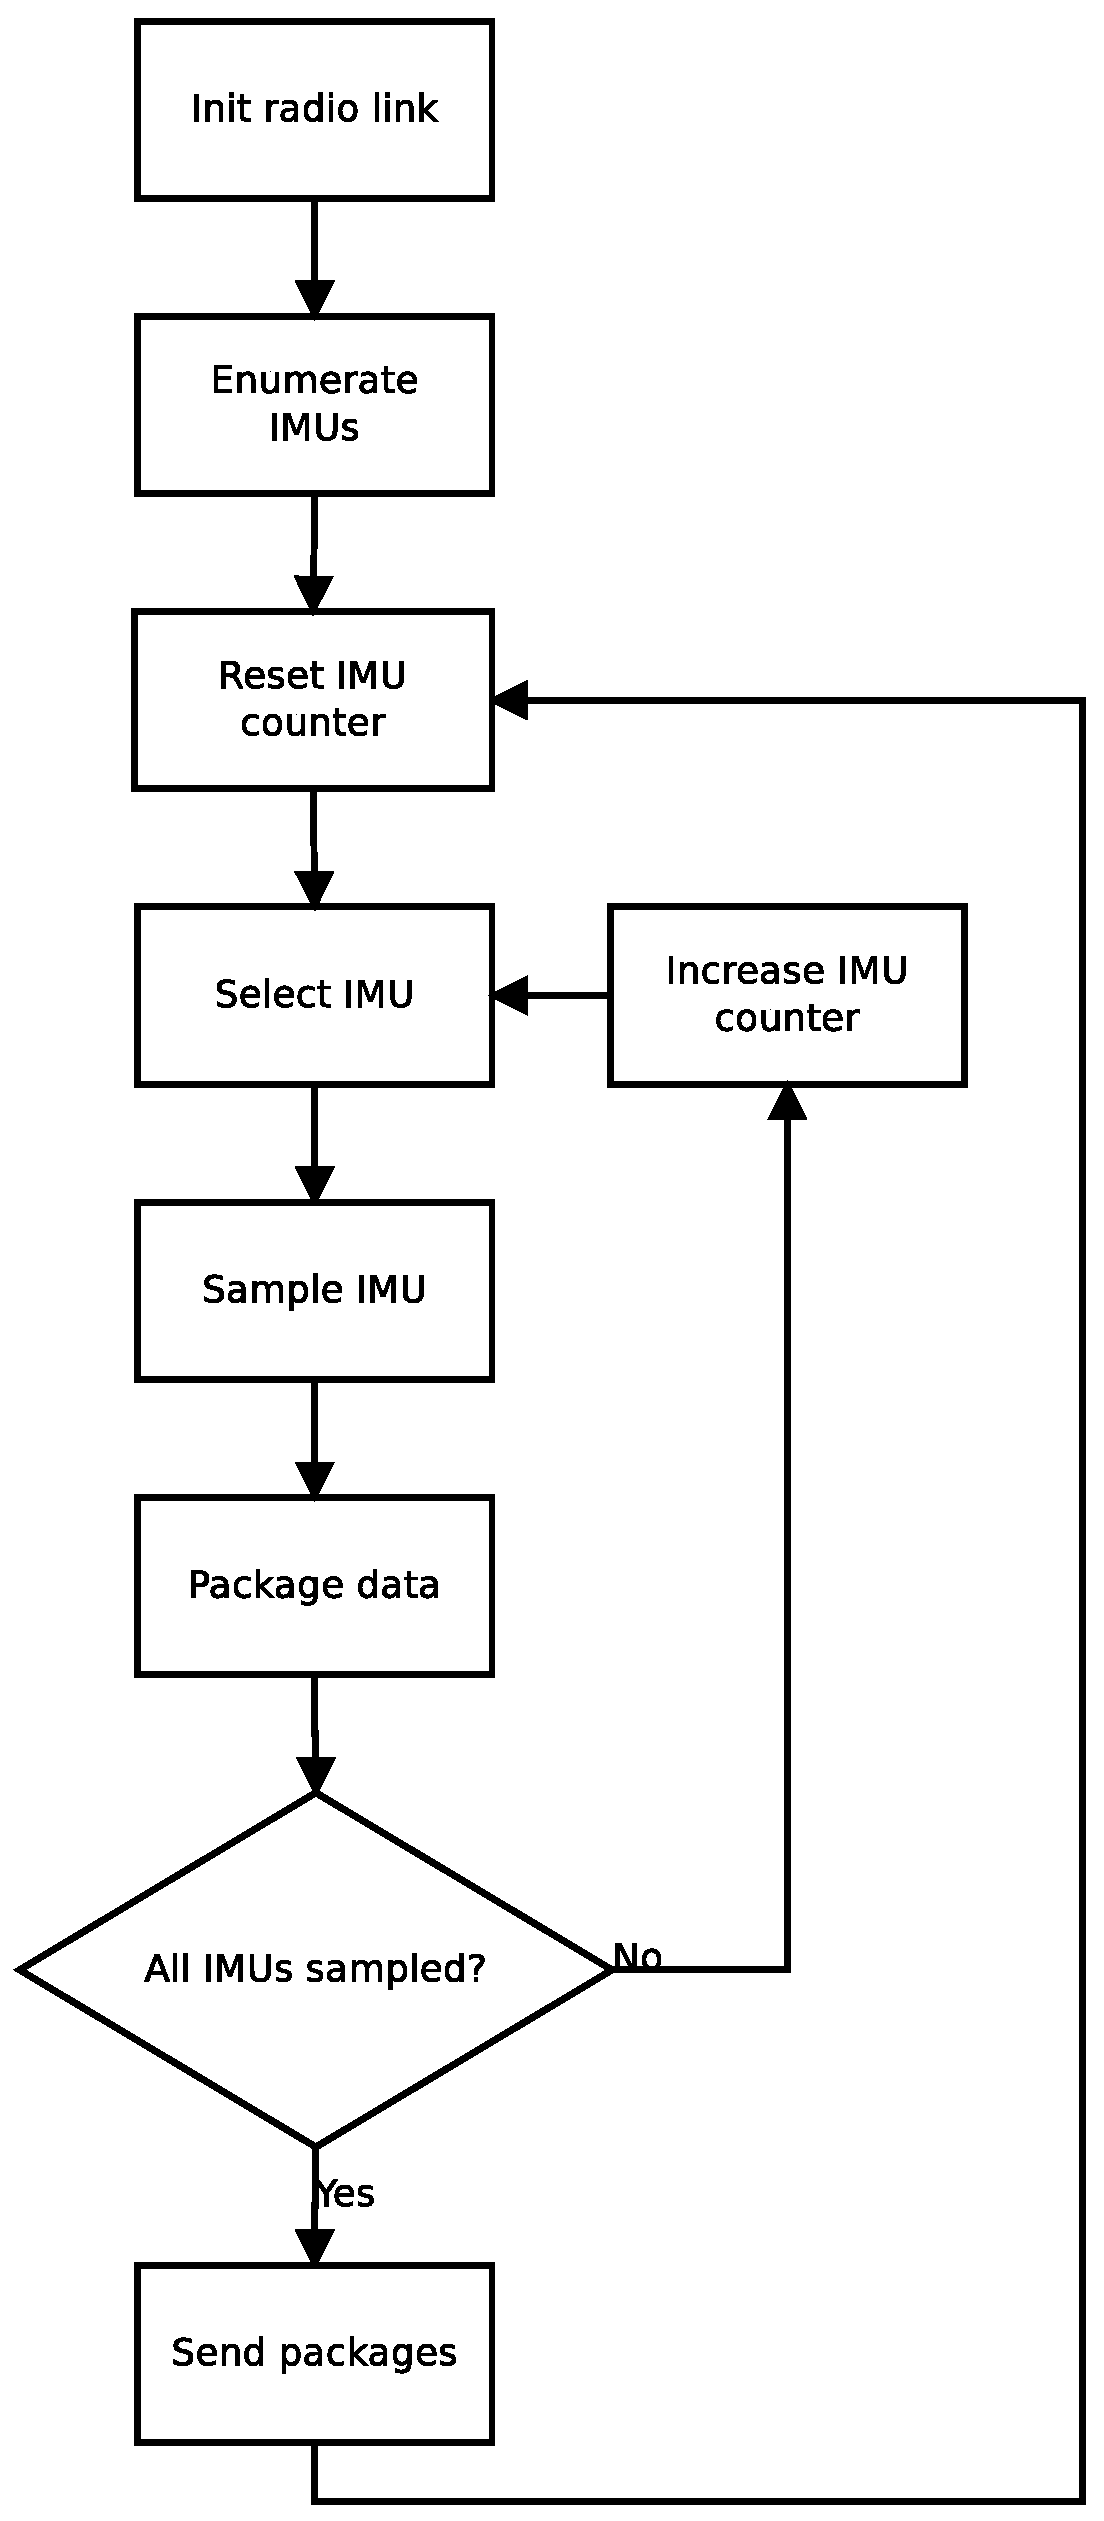
\includegraphics[scale=0.4]{micro.eps}
    \caption{Flow chart of motherboard micro controller code}
    \label{fig:pic3}
\end{figure}

\begin{figure}[H]
    \centering
    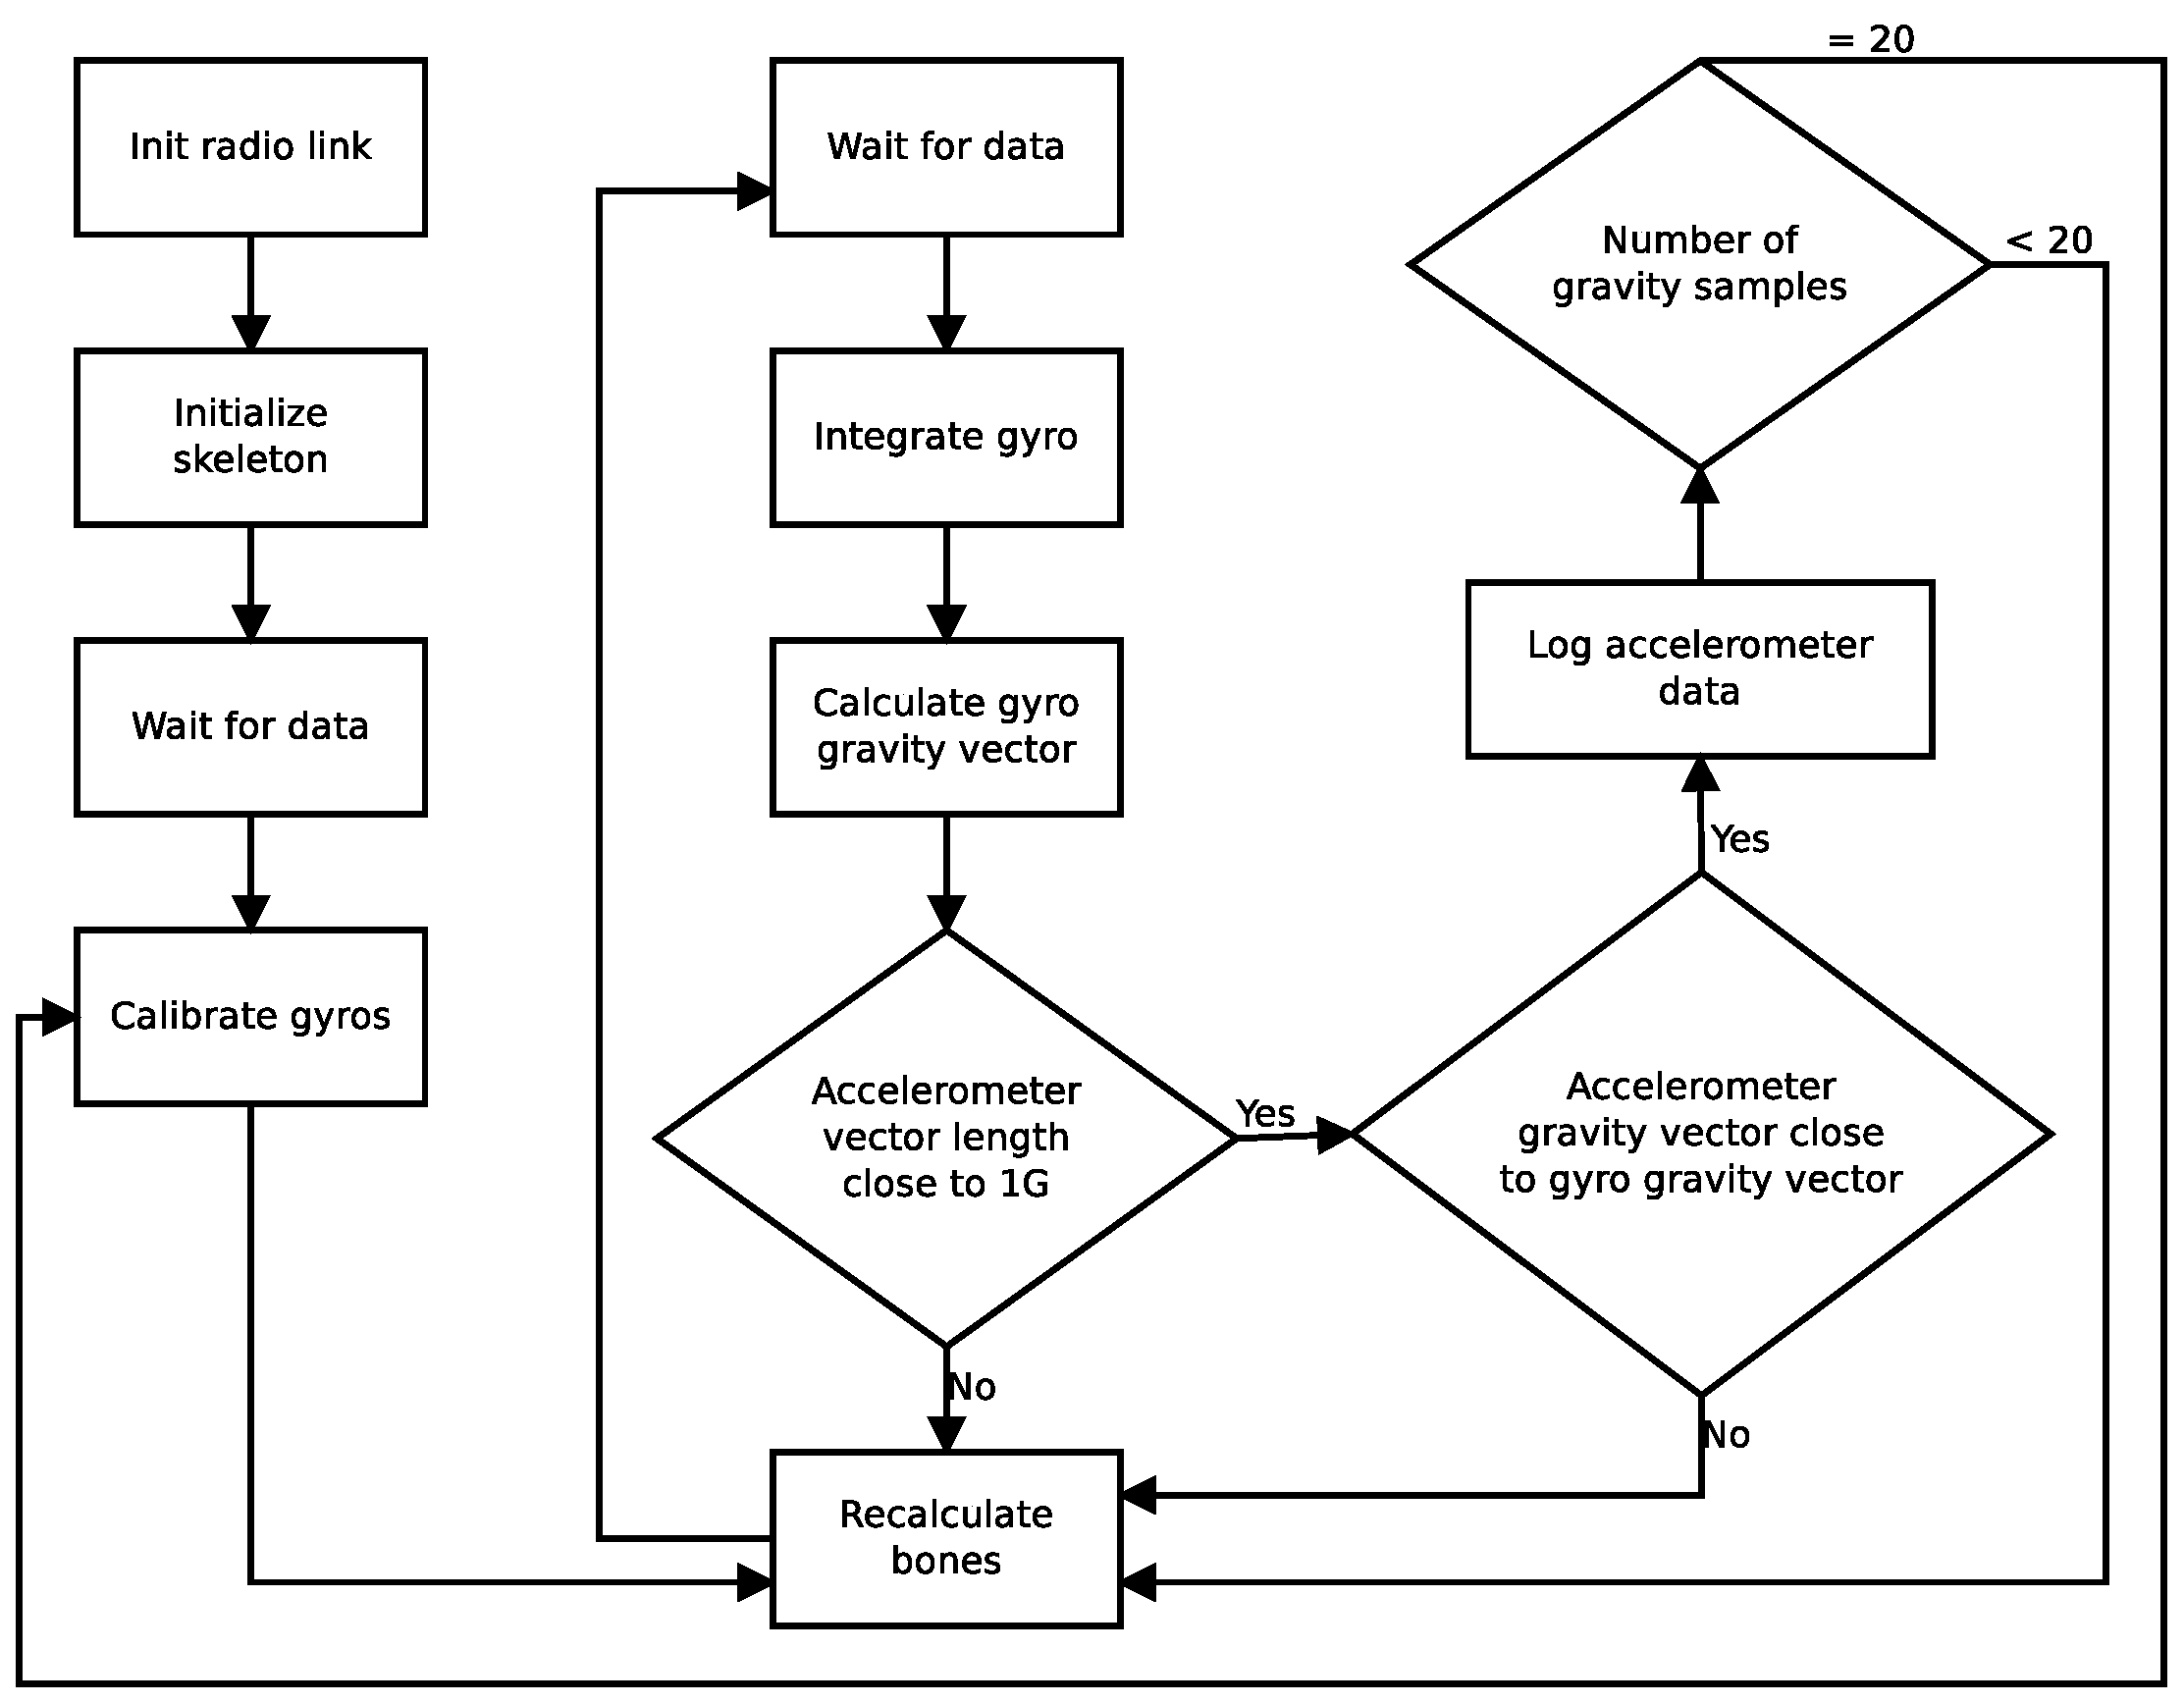
\includegraphics[scale=0.4]{pi.eps}
    \caption{Flow chart of host computer code}
    \label{fig:pic4}
\end{figure}


\subsection*{schematics}

\begin{figure}[H]
    \centering
    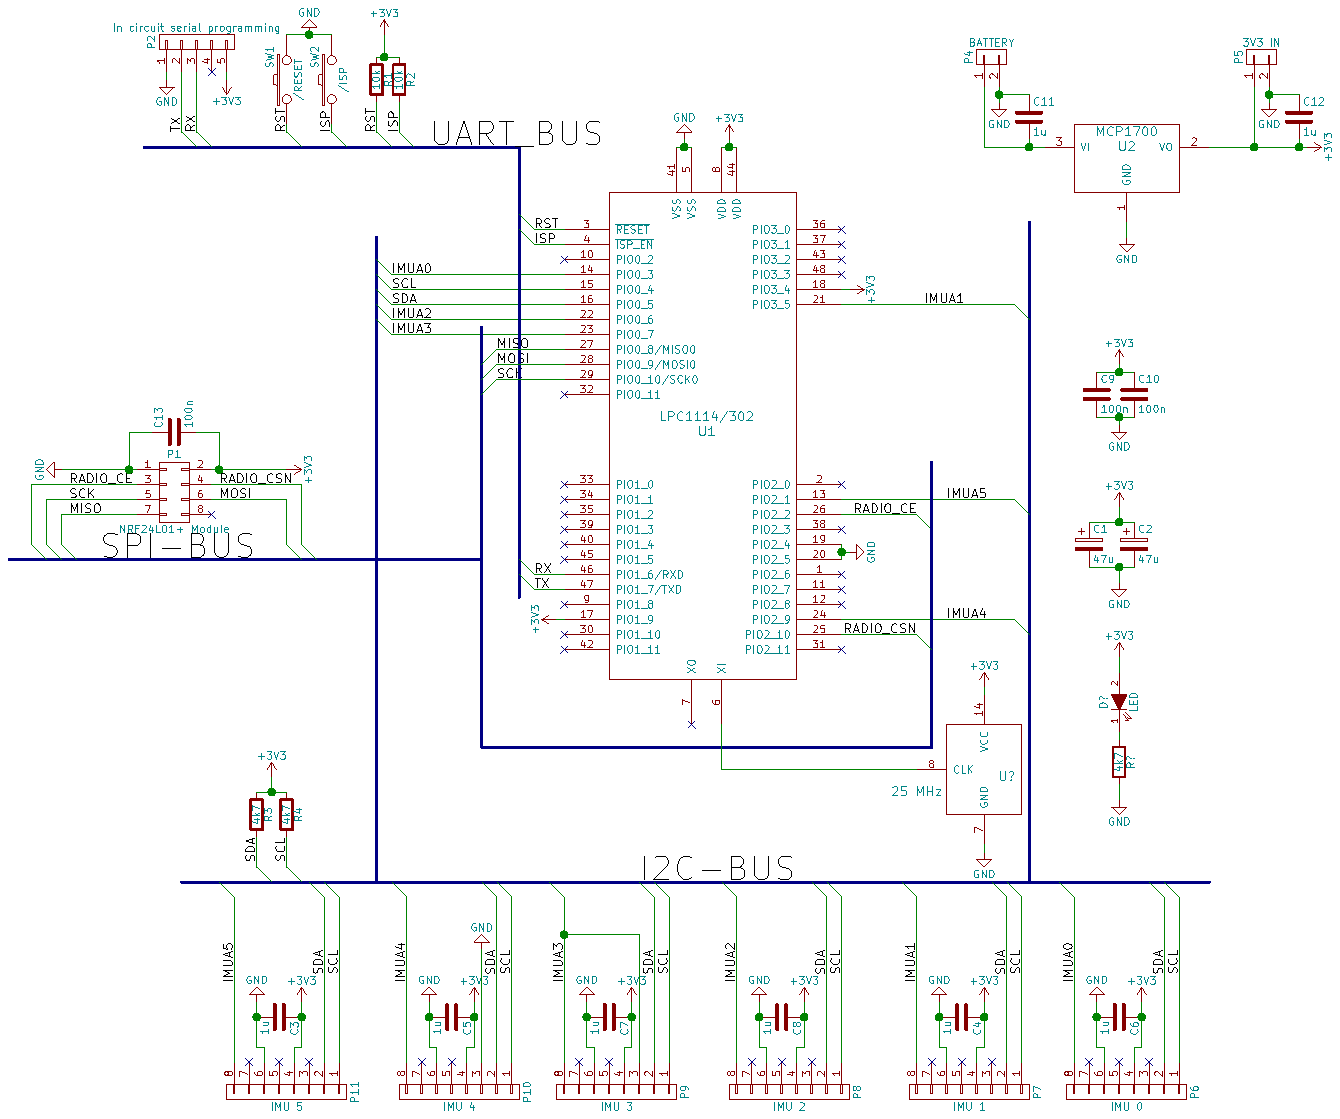
\includegraphics[scale=0.65]{mb_schematic.pdf}
    \caption{Motherboard schematic}
    \label{fig:pic5}
\end{figure}

\begin{figure}[H]
    \centering
    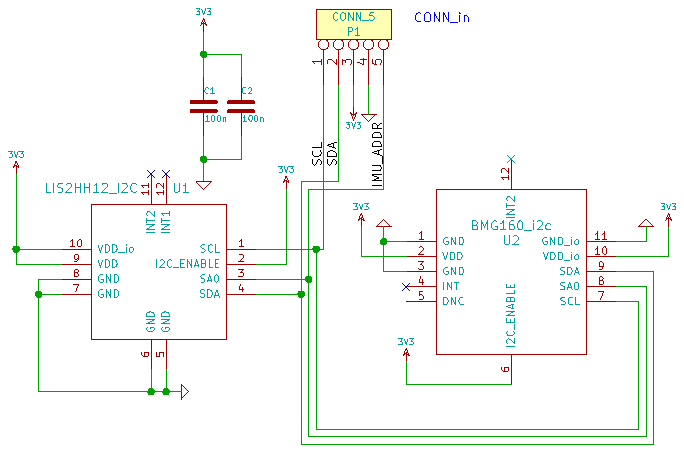
\includegraphics{imu_schematic.pdf}
    \caption{IMU board schematic}
    \label{fig:pic6}
\end{figure}


\section*{Data and Performance}

\begin{figure}[H]
    \centering
    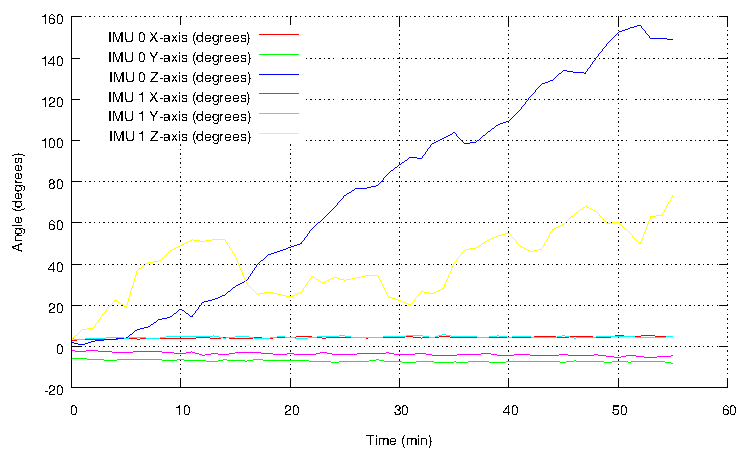
\includegraphics[scale=1.15]{drift.pdf}
    \caption{Stationary IMU drift over time}
    \label{fig:pic7}
\end{figure}

\begin{figure}[H]
    \centering
    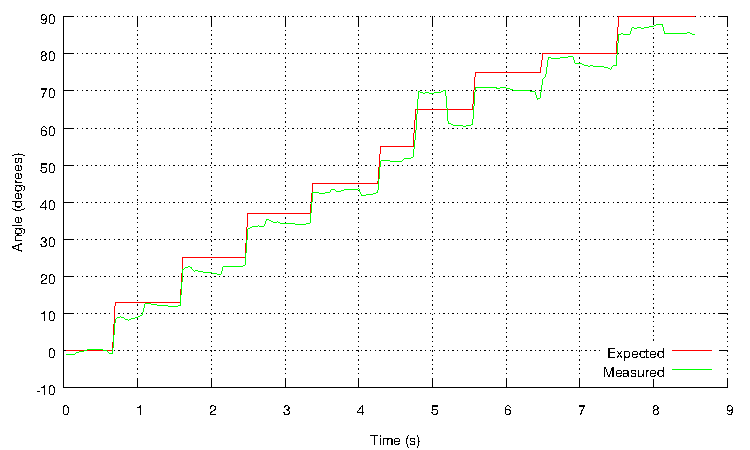
\includegraphics[scale=1.15]{stepped.pdf}
    \caption{Slow, stepped angle bend}
    \label{fig:pic8}
\end{figure}

\begin{figure}[H]
    \centering
    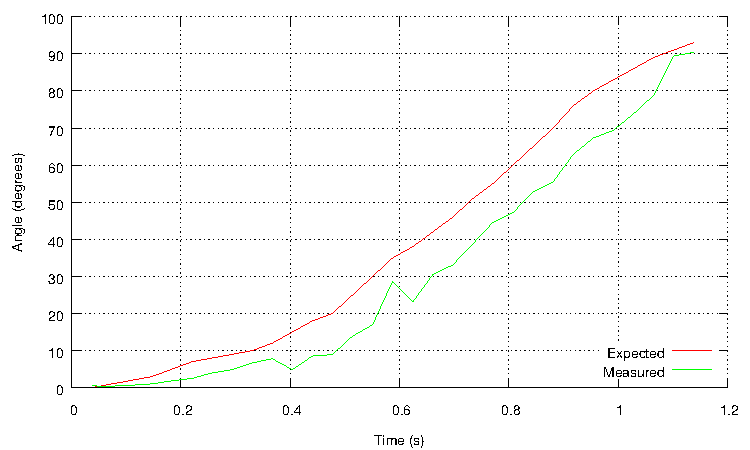
\includegraphics[scale=1.15]{fast_continuous.pdf}
    \caption{Fast, continuous bend}
    \label{fig:pic9}
\end{figure}

\section*{Individual reflection and Conclusion}
TO-DO

%%%%%%%%%%%%%%%%%%%%%%%%%%%%%%
%\newpage
%%\raggedright


\begin{thebibliography}{7}

\bibitem{kursp}
	The course web page,
	\textit{$https://people.kth.se/~msmith/II2302\_2016.html$}, fetched \date{\today{}}.

\bibitem{wiki}
	Motion Capture on Wikipedia,
	\textit{$www.en.wikipedia.org/wiki/Motion\_capture$}, fetched \date{\today{}}.


	


\end{thebibliography}
\end{document}

